The setup included a HeNe laser, tuning fork, lens, psd and some electronics. The laser were 
placed so that the laser beam hit the edge of the tuning fork. The tuning fork were placed in 
an holder that can adjust the position. Orthogonal to the tuning fork, a lens with focal length of 
50mm focus the scattered light on a PSD, see fig. \ref{fig:expSetupDiagram} and \ref{fig:expCompleteLive} for this setup.
The output signals from the PSD were connected to some electronics that transfer the output signals to a computer, see fig. \ref{fig:expCircuit}.

%1
\begin{figure}[h!]
	\centering
	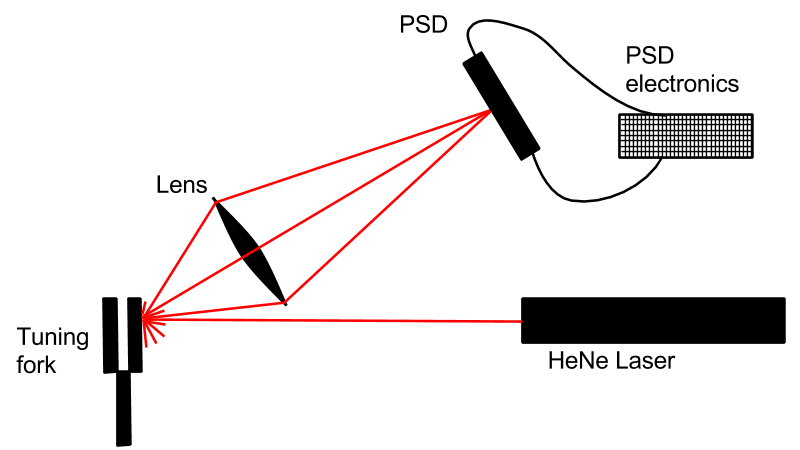
\includegraphics[width=0.8\textwidth]{img/expSetupDiagram}
	\caption{Diagram of the setup for measuring the movement of the tuning fork.}
	\label{fig:expSetupDiagram}
\end{figure}

%2.
\begin{figure}[h!]
	\centering
	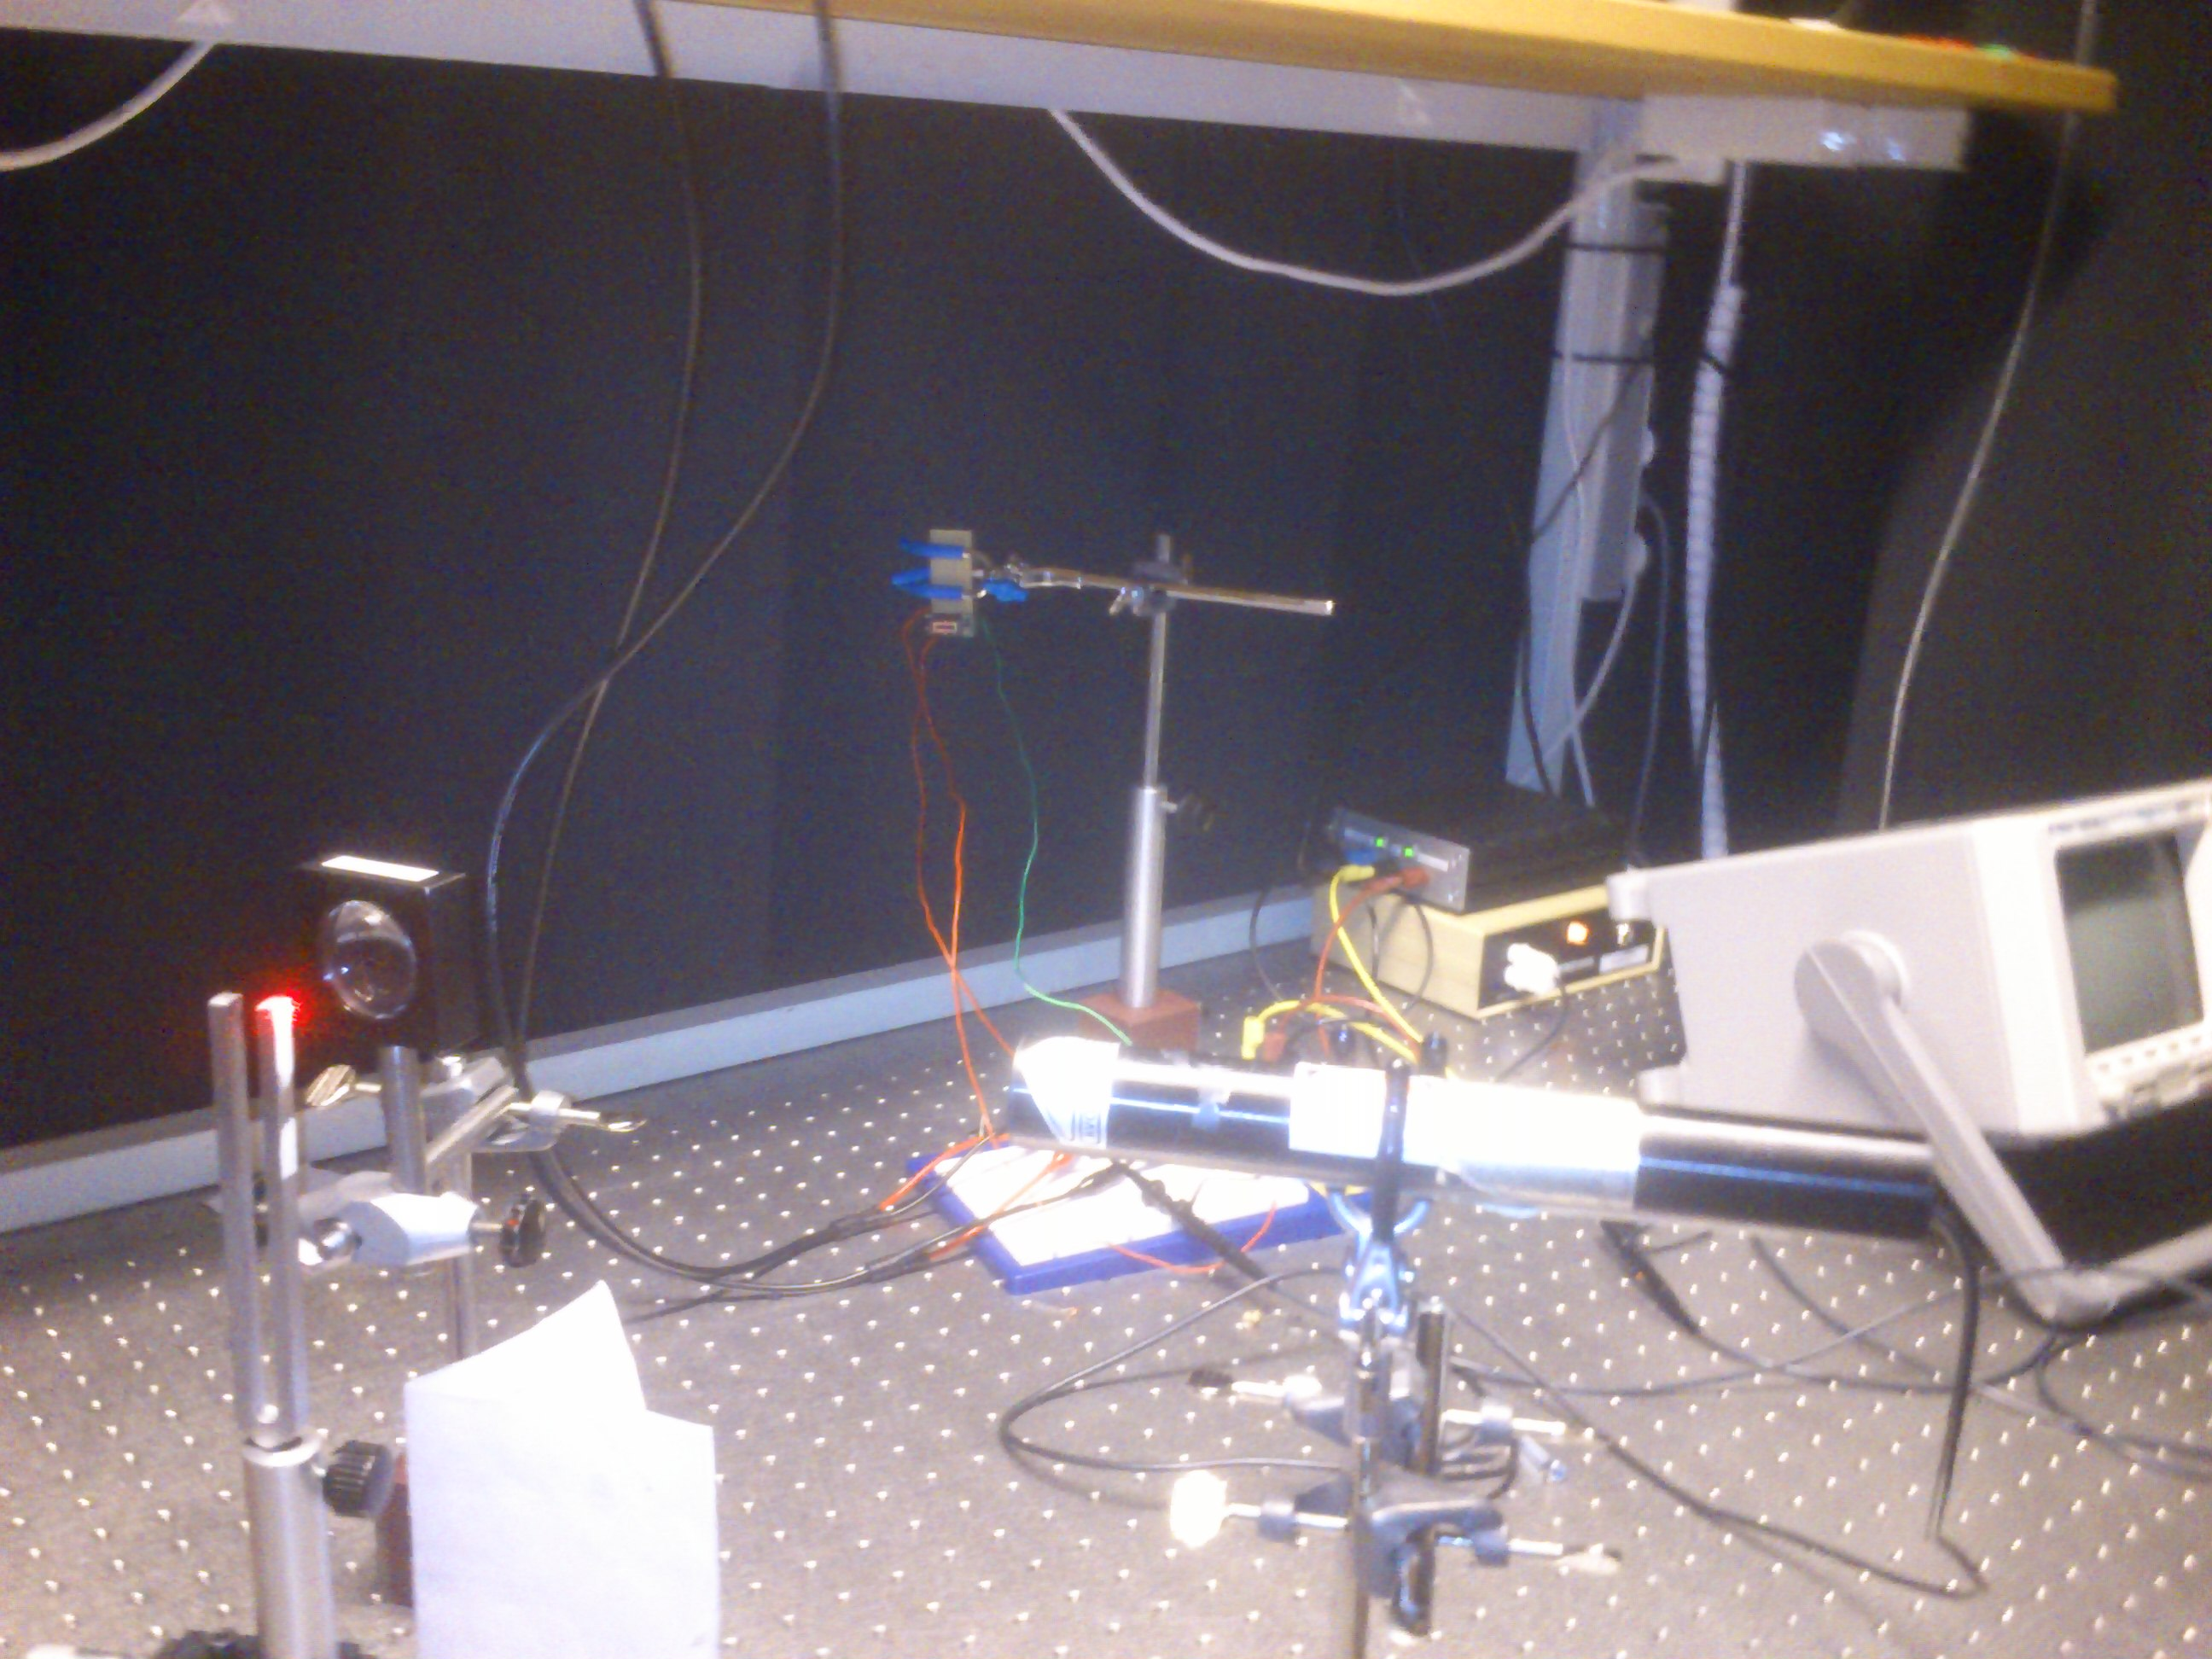
\includegraphics[width=0.8\textwidth]{img/expCompleteLive}
	\caption{The setup with the laser pointed at the tuning fork and a lens that collects the scattered light onto the PSD}
	\label{fig:expCompleteLive}
\end{figure}

%3
\begin{figure}[h!]
	\centering
	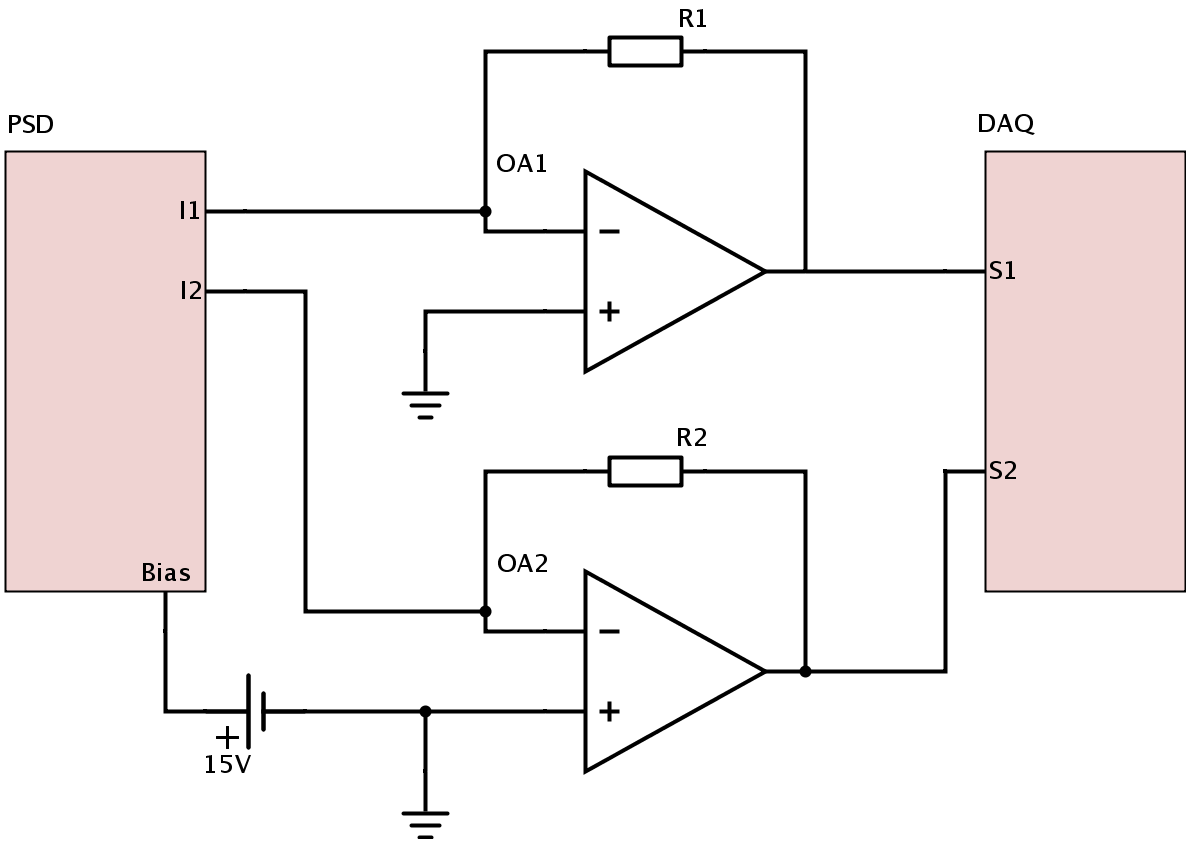
\includegraphics[width=0.8\textwidth]{img/expCircuit}
	\caption{The circuit design to transform and amplifies the current signal from the PSD to a voltage signal for the DAQ that sends it on to the computer.}
	\label{fig:expCircuit}
\end{figure}

%4

In order to be calibrate the output signal an accurate slide is used to see what signal correspond to what signal on the output, see fig \ref{fig:expCalibrateLive}.
\begin{figure}[h!]
	\centering
	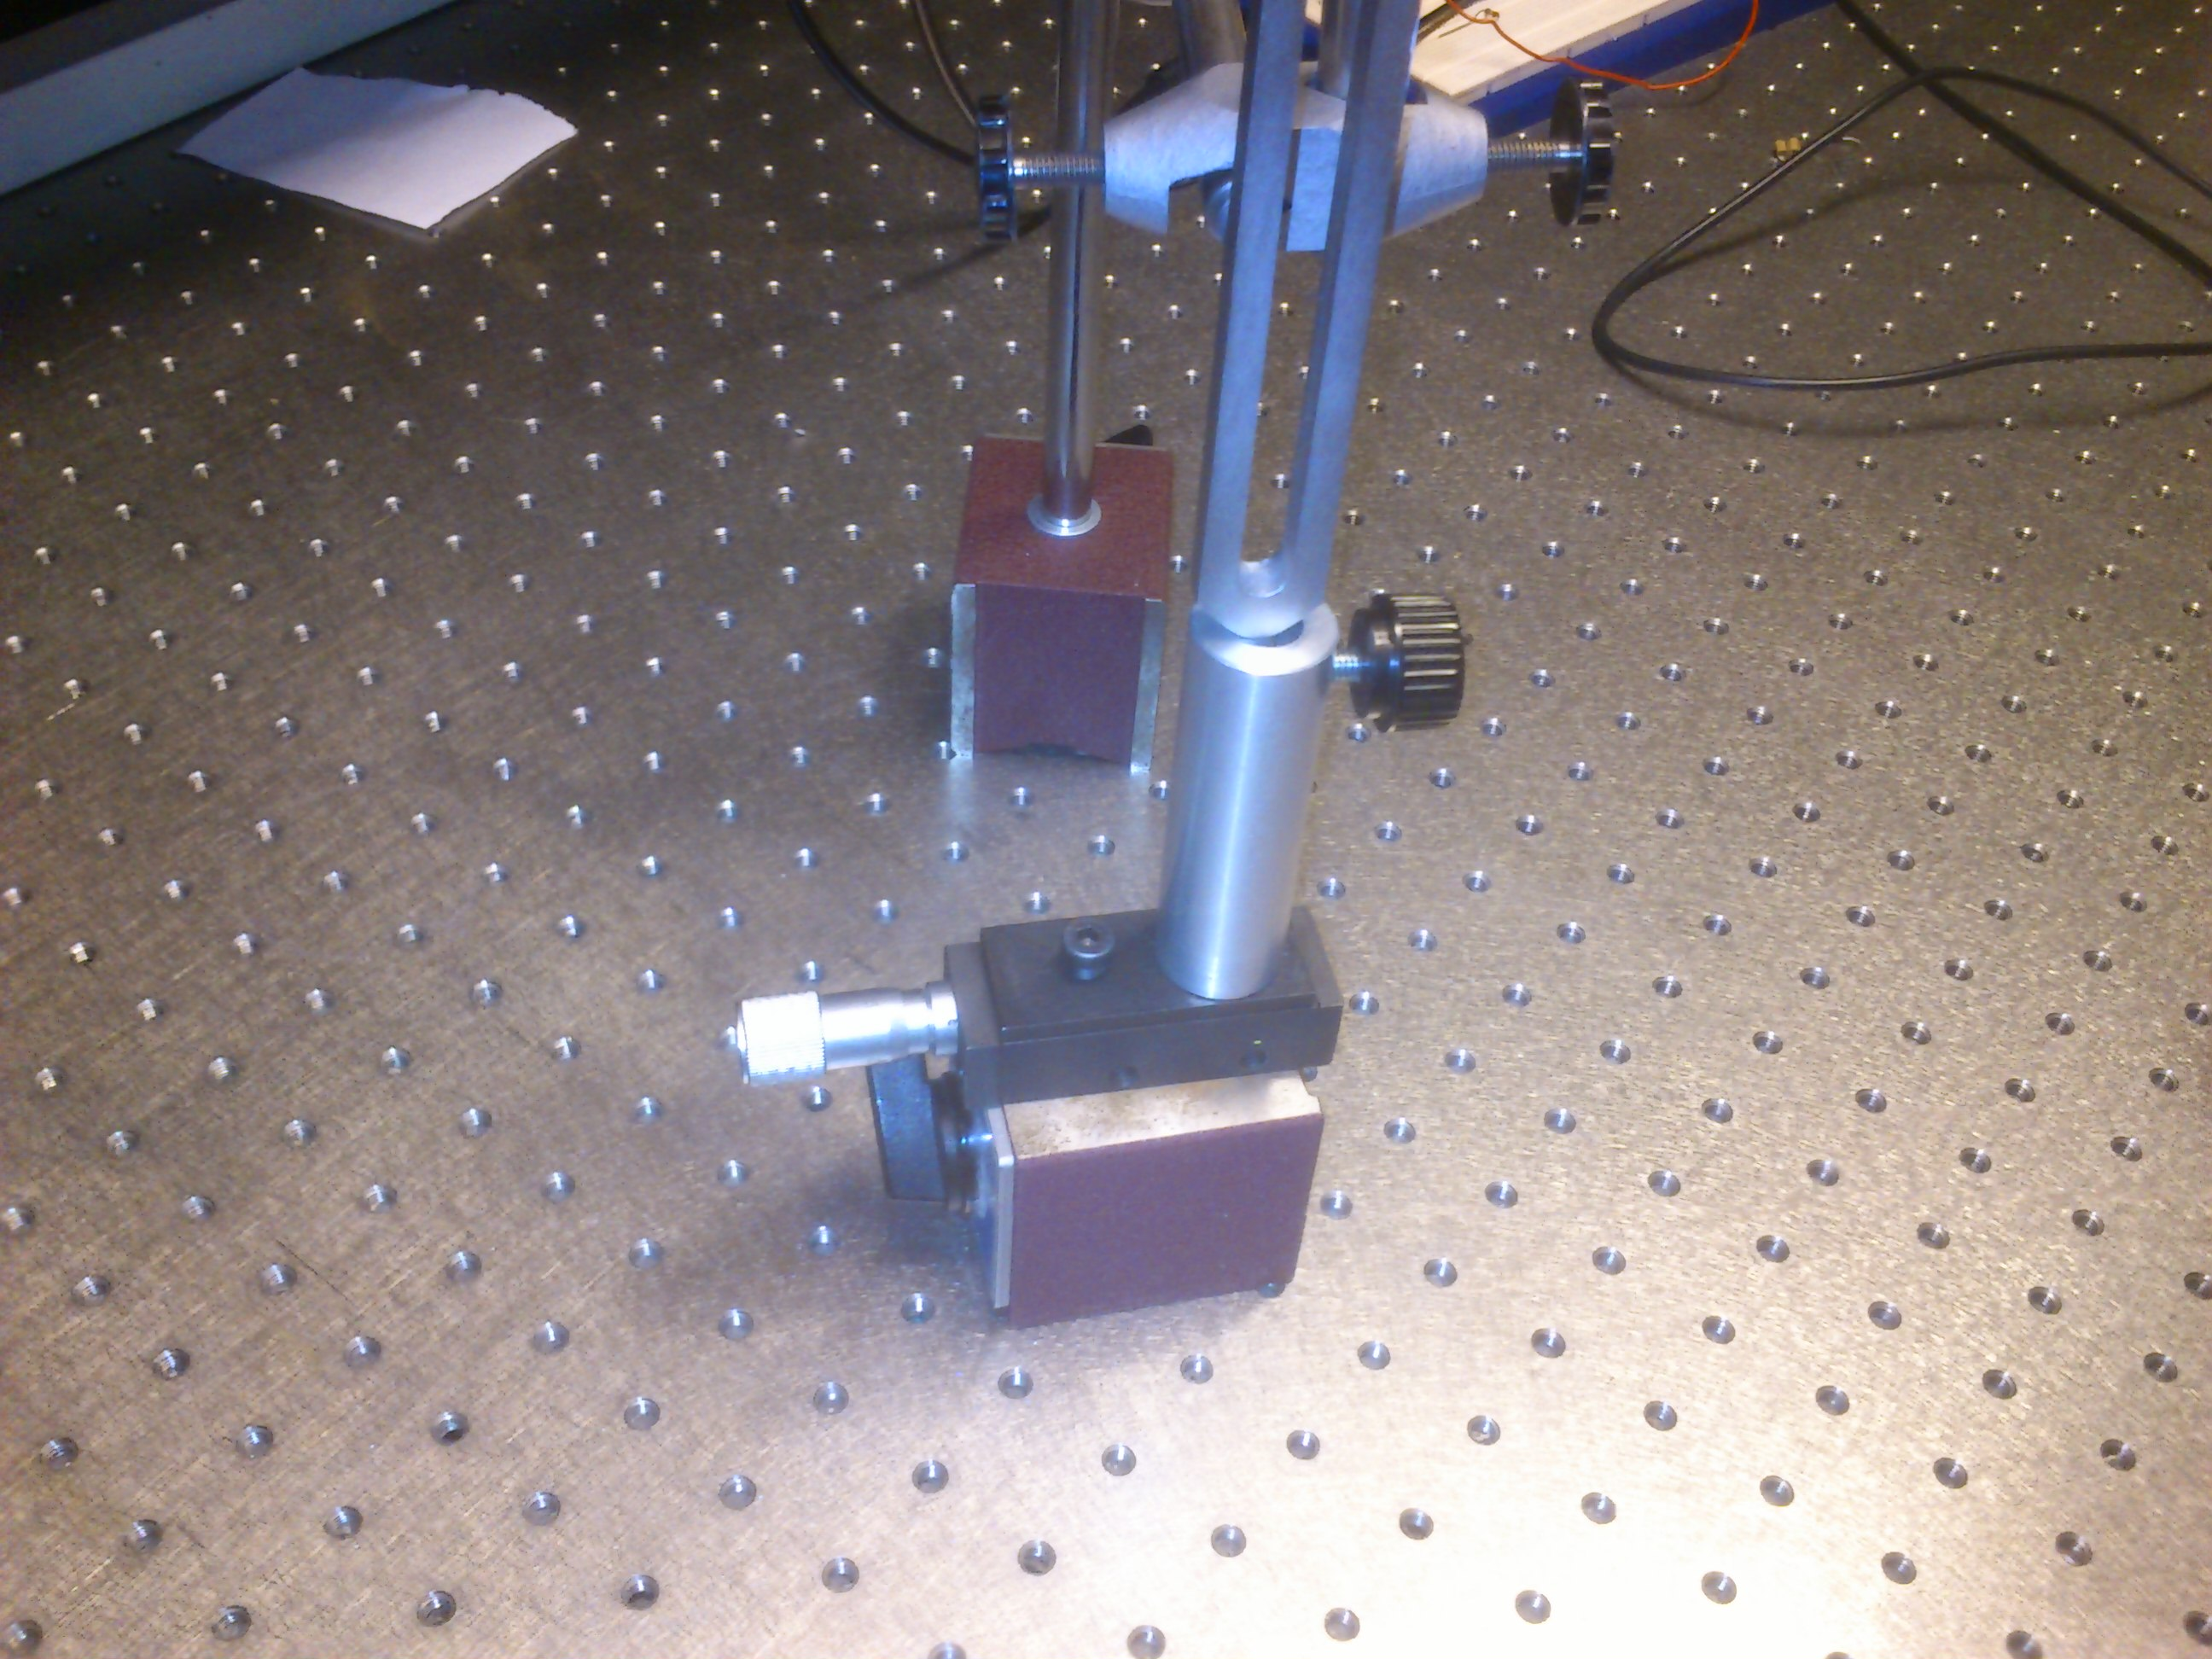
\includegraphics[width=0.8\textwidth]{img/expCalibrateLive}
	\caption{The position of the tuning fork can be adjusted using this slide. This is used to calibrate what movement on the PSD corresponds to what movement on the tuning fork.}
	\label{fig:expCalibrateLive}
\end{figure}

